
In this section we briefly recall the model-based control with regression trees algorithm (mbCRT) proposed in \cite{Behl201630} to synthesize optimal control strategies. 
We provide a general formulation that is suitable for any cyber-physical system.
This will be useful in the next section to introduce our new algorithm. 

\subsection{Data-driven one-step look ahead predictive model}
\label{sec:mbcrt}

\begin{figure}
\centering
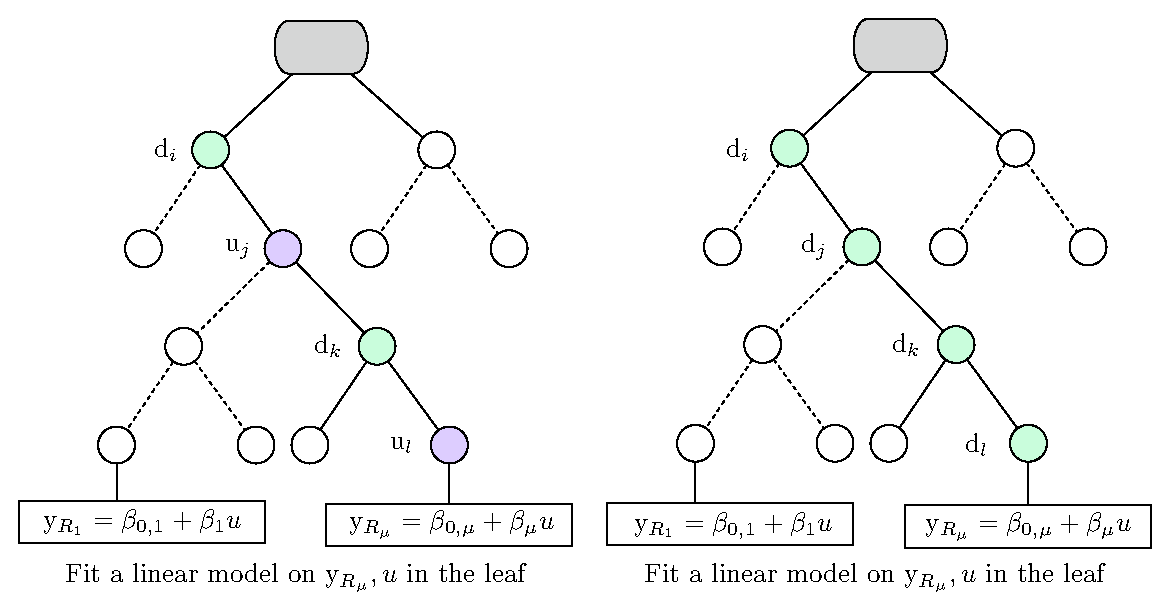
\includegraphics[width=0.9\columnwidth]{Figures/sep_vars.eps}
   \caption{Example of a regression tree not suitable for control due to the mixed order of $\mathcal{X}_c$ and $\mathcal{X}_d$ (left). Example of a tree structure obtained for the mbCRT algorithm. The separation of variables allows using the linear model in the leaf to depend only on the control variables (right).}
   \captionsetup{justification=centering}
   \label{fig:training}
\end{figure}

The \emph{model based Control with Regression Trees (mbCRT)} uses the separation of variables introduced in Sec. \ref{sec:problem}.
The model construction is illustrated in Fig.~\ref{fig:training} -- a regression tree is trained only on disturbance features in $\mathcal{X}_d= \{ \mathrm{d_1,\ldots,d_{s-m}} \} $ to predict the output variable $\mathrm{y}$. Without any loss of generality, we consider only single response variable. 
Multiple trees can be considered for multiple response variables as we do for the case study in Sec.~\ref{sec:case}. 
After learning a regression tree, a linear regression model

\begin{equation}\label{eq:linear_regression_leaf}
\mathrm{y}_{R_\mu} = \beta_{0,\mu} + \beta_\mu u
\end{equation}
is fitted using the subset of samples present in every leaf of the tree, where $\mathrm{y}_{R_\mu}$ is the predicted response in region $R_\mu$ of the tree using all the features in $\mathcal{X}_d$, and $\beta_{0,\mu}\in\mathbb{R}$ and $\beta_\mu\in\mathbb{R}^{1\times m}$. 
Separation of variables allows to use the forecast of the disturbances in $\mathcal{X}_d$ to navigate to the appropriate region $R_\mu$ and use the linear regression model \eqref{eq:linear_regression_leaf} with only the control variables in it as the valid prediction model for that time-step.
The linear model approximation in the leaves is validated in \cite{Behl201630}.
The left part of Fig. \ref{fig:training} shows the case where all the features in $\mathcal{X}$ are used to train the trees. 
In such a tree, control variables are used as the splitting variables at several nodes. 
As a consequence, as already explained in Sec.~\ref{sec:problem}, this does not allow to set up an MPC-like optimization problem, since inputs values are not available a priori to go through the tree and determine the correct region $R_\mu$.

\subsection{Data-driven optimal control}
Given $p$ response variables and $s$ training features, of which there are $m$ input and $s-m$ disturbance variables, $p$ regression trees are built to create models as in \eqref{eq:linear_regression_leaf} for every response variable. Then, at each time-step $t$ the following quadratic optimal control problem is solved:

\begin{equation}\label{eq:mbCRT}
\begin{aligned}
& \underset{u_t \in \mathcal{X}_c}{\text{minimize}} & &  y^\top_t \mathrm{Q}\, y_t + u^\top_t \mathrm{R}\, u_t              \\
& \text{subject to }                                & &  \mathrm{y}_{1,t}    =   \beta_{0,i_1} + \beta_{i_1}u_t     \\
&                                                   & &  \mathrm{y}_{2,t}    =   \beta_{0,i_2} + \beta_{i_2}u_t     \\
&                                                   & &  \vdots                                                         \\
&                                                   & &  \mathrm{y}_{p,t}    =   \beta_{0,i_p} + \beta_{i_p}u_t     \\
&                                                   & &  u_t                \in  \mathcal{\bar U}.                       \\
\end{aligned}
\end{equation}
The optimal control input $u(t) = u^*_t$ is applied to the system, and the optimization is repeated at $t+1$. $\mathrm{Q}$ and $\mathrm{R}$ are the design parameters to trade-off the quadratic objective function components. Different objective functions can be chosen, for example linear or non-linear, as well as different models in the leaves instead of \eqref{eq:linear_regression_leaf}, decreasing or increasing the complexity of the problem.
